% Chapter 3

\chapter{Teoria de Antenas} % Main chapter title
\label{chap:Chapter3} % For referencing the chapter elsewhere, use \ref{chap:Chapter3} 

%----------------------------------------------------------------------------------------
\section{Teoria Básica de Antenas}
Uma antena é definida como "um dispositivo geralmente metálico (com haste ou fio) para irradiar ou receber ondas de rádio" \parencite{Balanis2016}, ou seja, uma antena, é o dispositivo que permite a transição entre o meio que a rodeia e o equipamento, que se pode observar na Figura \ref{fig:antena transicao}. 
Este dispositivo é um transdutor que converte energia elétrica em ondas eletromagnéticas ou vice versa, sendo que é uma antena de transmissão, se converter um sinal elétrico num sinal eletromagnético e é uma antena de receção, se converter um sinal eletromagnético em sinal elétrico. 

\begin{figure}[h]
\centering
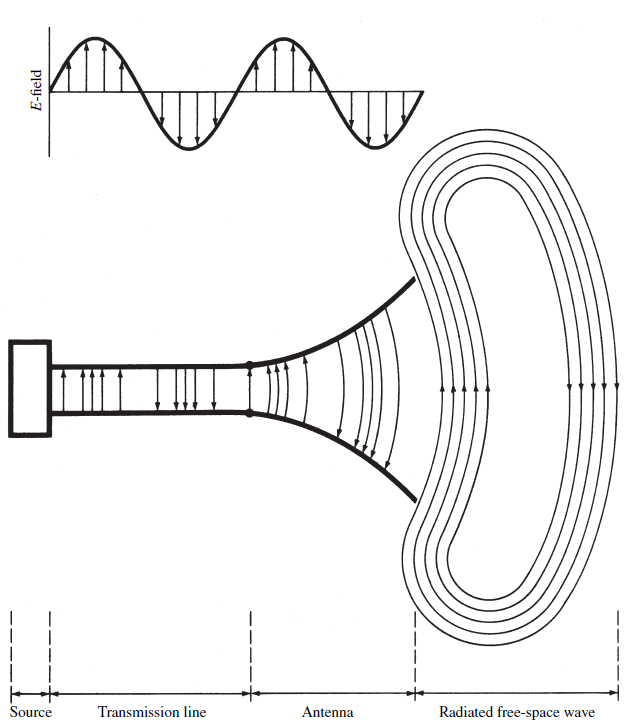
\includegraphics[scale=0.6]{chapters/ch3/assets/Antenna_transicao}
\decoRule
\caption[Antena como meio de transição]{Antena como um meio de transição (Figura 1.1 - \cite{Balanis2016})}
\label{fig:antena transicao}
\end{figure}

\subsection{Tipos de Antenas}
Neste subcapítulo irá ser introduzido de uma forma breve, os vário tipos de antenas, a sua utilização e vantagens entre estes. 

\subsection*{Antenas de Fio}
Estas antenas são umas das mais antigas, que apresentam uma configuração mais simples, como se pode observar na Figura \ref{fig:wire antenna}, sendo apenas constituídas por um fio que pode variar na sua dimensão e na sua forma e ainda podem ser utilizadas nas mais variadas aplicações. Podem tomar uma forma aleatória, desde um fio direito (dipolo) até um fio com as mais diversas formas. \par 
As antenas de fio podem ser encontradas nos mais variados locais, desde aeronaves, carros ou navios a edifícios.

\begin{figure}[h]
\centering
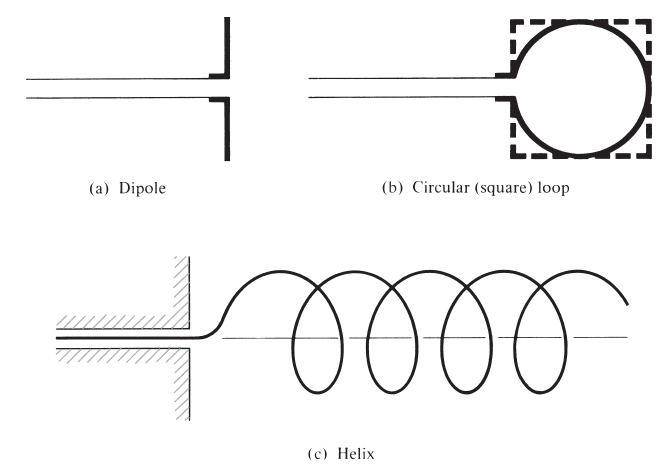
\includegraphics[scale=0.6]{chapters/ch3/assets/wire_antenna}
\decoRule
\caption[Antena de Fio]{Exemplos de vários tipos de antenas de fio (Figura 1.3 - \cite{Balanis2016})}
\label{fig:wire antenna}
\end{figure}

\subsection*{Antenas de Abertura}
Os campos no fim de um guia de ondas aberto não são uniformes devido a esta mesma abertura, assim, para este caso, assume-se que os campos são iguais a como se o guia de ondas continuasse fechado. As antenas de abertura entram quando se pretende aumentar a diretividade à saída do guia, abrindo as extremidades do mesmo de forma a dar uma forma como se observa na Figura \ref{fig:aperture antenna2}. Este tipo de antenas, em especifico as antenas de abertura piramidais, são utilizadas para alimentar ou calibrar grandes antenas de prato.\par
Assim sendo, as antenas de abertura são utilizadas para frequências mais elevadas, especificamente em frequências de micro-ondas e podem ser aplicadas nas mais variadas formas geométricas, como retangulares, elípticas, circulares, piramidais, entre outras.

\begin{figure}[h]
\centering
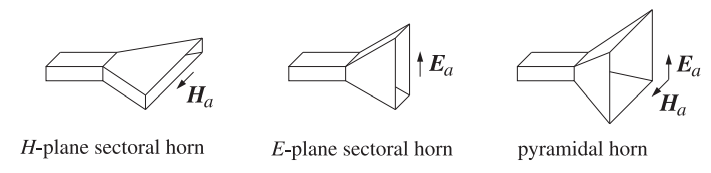
\includegraphics[scale=0.6]{chapters/ch3/assets/aperture_antenna2}
\decoRule
\caption[Antena de Abertura]{Antenas de abertura no plano H, E e piramidal}
\label{fig:aperture antenna2}
\end{figure}


\subsection*{Antenas de \textit{Microstrip}}
Uma antena \textit{microstrip}, conhecida como antena impressa, é um tipo de antena que está inserida numa placa de circuito impresso e funciona como uma antena interna.\par
Hoje em dia são utilizadas em aplicações comerciais, tendo como as suas maiores vantagens o facto de serem baratas e simples de manufaturar e apresentarem um tamanho reduzido. Este tipo de antenas são aplicadas em frequências \gls{UHF}.\par 
A sua construção consiste num \textit{patch} metálico sobre um substrato. Este \textit{patch} pode apresentar as mais variadas formas como representado na Figura \ref{fig:microstrip}, sendo as retangulares e circulares as mais comuns. Têm ainda as vantagens de serem impressas em superfícies com as mais variadas formas, sendo robustas e versáteis nos parâmetros da sua frequência de ressonância, polarização e impedância (\cite{Balanis2016}).

\begin{figure}[h]
\centering
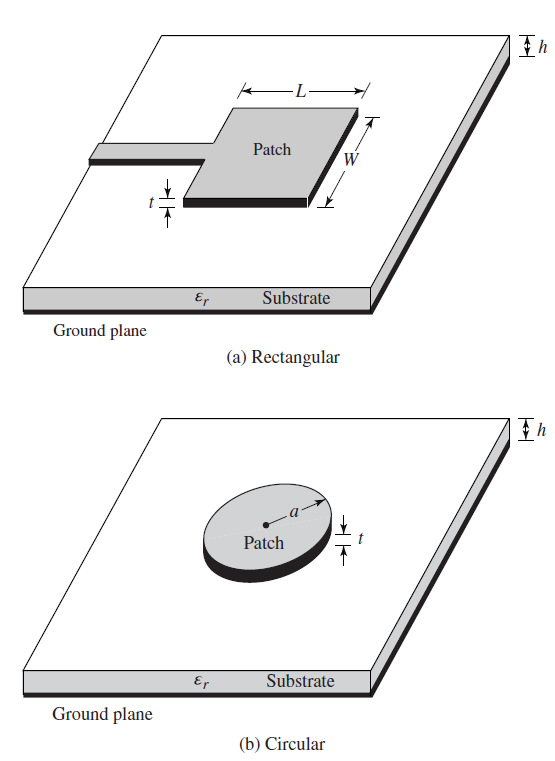
\includegraphics[scale=0.6]{chapters/ch3/assets/microstrip}
\decoRule
\caption[Antena \textit{Microstrip}]{Exemplos de duas configurações de \textit{patches} diferentes (Figura 1.5 - \cite{Balanis2016})}
\label{fig:microstrip}
\end{figure}

\subsection*{Antenas de Matrizes}
As antenas de matrizes surgem nas aplicações em que é necessário mais que um elemento. Consegue-se assim agrupar vários elementos de forma a obter as características pretendidas. Algumas alterações às caraterísticas que se conseguem com este tipo de antenas antenas são o aumento de ganho, alterar o diagrama de radiação, determinar a direção de chegada de um sinal ou maximizar o \gls{SINR}\footnote{\gls{SINR} é um indicador de qualidade de transmissão ajustado a comunicações móveis devido à interferência de outros utilizadores ser mais significativa \parencite{Jeske2004}.}.

\subsection*{Antenas de Lente}
Este tipo de antenas utiliza as propriedades de convergência e divergência das lentes para a receção ou transmissão de sinal. O tamanho da lente a ser utilizada depende da frequência - quanto maior for a frequência, menor a lente. Dito isto, é mais favorável usar este tipo de antenas em frequências mais altas, visto que a lente será menor. As suas aplicações são semelhantes às das refletoras parabólicas, especificamente quando usadas em frequências mais altas e que necessitem de mais largura de banda.

\subsection*{Antenas Refletoras}
As antenas refletoras existem desde o final do século XIX, no entanto começaram a ser aplicadas em radares na Segunda Guerra Mundial e a partir do final do século XX em comunicações espaciais. Estas aplicações devem-se à sua capacidade de transmissões a grandes distâncias. Podem-se apresentar nas mais diversas formas, como plano refletor, refletor curvilíneo, entre outros.\par 
O seu modo de funcionamento baseia-se na convergência da energia numa direção como demonstrado na Figura \ref{fig:reflector}, o que leva, para além de um grande alcance, a uma grande diretividade.

\begin{figure}[h]
\centering
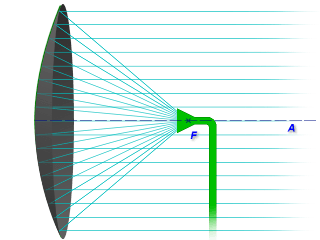
\includegraphics[scale=0.6]{chapters/ch3/assets/reflector}
\decoRule
\caption[Antena Refletora]{Funcionamento de uma Antena Refletora}
\label{fig:reflector}
\end{figure}

\subsection{Parâmetros Fundamentais}
Neste subcapítulo vão ser discutidos os parâmetros fundamentais para o funcionamento de uma antena e a sua \textit{performance}. Grande parte dos parâmetros estão definidos no \parencite{IEEE1983}.

\section{Simulação de uma Antena}


\subsection{Para Sinais DVB-T}

